Listing problems are common problems in combinatorics. In general, listing problems 
focus on enumerating the objects of a given finite set in some specific order. The listing problem in this thesis 
will be termed \emph{The Canonical Ladder Listing Problem}. This problem asks, given all $n!$ permutations of order $n$, is there an efficient algorithm for listing 
one optimal ladder per permutation? In other words, is there an easy way to transition from one ladder to the next until all $n!$ ladders 
have been listed? The problem is stated as follows: Let $S_{n}$ be the set of all $n!$ permutations of order $n$. 
Let the \emph{canonical representative} be the root ladder from each permutation's corresponding $OptL\{\pi\}$. Let $L_{n}$ be the set of 
all $n!$ root ladders. Refer to Figure~\ref{Fig:Route} for the root ladder for $(3,5,4,1,2)$.
\begin{figure}[h]
	\centering
	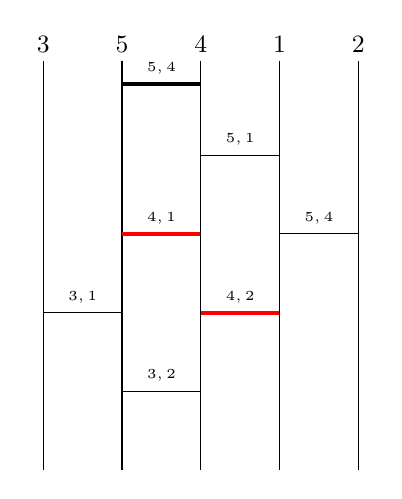
\begin{tikzpicture}
		\draw(0, 0) to (0, 5.2);

			
			\node at(.5, 2.2){\tiny{$3,1$}};
			\draw(0, 2) to (1, 2);
		\draw(1, 0) to (1, 5.2);
			\node at(1.5, 5.1){\tiny{$5,4$}};
			\draw[line width=.5mm](1, 4.9) to (2, 4.9);

			\node at(1.5, 3.2){\tiny{$4,1$}};
			\draw[line width=.5mm, red](1, 3.0) to (2, 3.0);

			\node at(1.5, 1.2){\tiny{$3,2$}};
			\draw(1, 1) to (2, 1);
	%		\node at(.75, .9){\tiny{$3,2$}};
	%		\draw(.5, .7) to (1, .7);
		\draw(2, 0) to (2, 5.2);

			\node at(2.5, 4.2){\tiny{$5,1$}};
			\draw(2, 4) to (3, 4);


			\node at(2.5, 2.2){\tiny{$4,2$}};
			\draw[line width=.5mm, red](2, 2) to (3, 2);
			%\node at(1.25, 2.1){\tiny{$4,1$}};
			%\draw[line width=.5mm, red ](1, 1.9) to (1.5, 1.9);
			%\node at(1.25, 1.3){\tiny{$5,2$}};
			%\draw(1, 1.1) to(1.5, 1.1);
		\draw(3, 0) to (3, 5.2);
			
			\node at(3.5, 3.2){\tiny{$5,4$}};
			\draw(3, 3.0) to (4, 3.0);	
		%\node at(1.75, 1.7){\tiny{$4,2$}};
			%\draw[line width=.5mm, red ](1.5, 1.5) to (2, 1.5);
			%\node at(1.75, .9){\tiny{$5,4$}};
			%\draw[line width=.5mm, red ](1.5, .7) to (2, .7);
		\draw(4, 0) to (4, 5.2);


		\node at(0.0, 5.4){\small{$3$}};
		\node at(1, 5.4){\small{$5$}};
		\node at(2.0, 5.4){\small{$4$}};
		\node at(3, 5.4){\small{$1$}};
		\node at(4, 5.4){\small{$2$}};
	\end{tikzpicture}
	\caption{The root ladder for $(3,5,4,1,2)$}
	\label{Fig:Route}
\end{figure}
A \emph{change} 
is defined as the insertion or deletion of at least one bar from a ladder in $L_{n}$. The goal is 
to list $L_{n}$ by changing $l_{i}\in L_{n}$ to get to $l_{i+1} \in L_{n}$.\par
In this thesis, two listing algorithms are used to list $L_{n}$. The first of these listing algorithms 
is a modification of the {\sc Steinhaus-Johnson-Trotter} permutation listing algorithm~\cite{A25}.
This algorithm is termed {\sc ModifiedSJT}.
The second listing algorithm is influenced by Effler and Ruskey's algorithm~\cite{A26}. 
This second ladder listing algorithm is termed the {\sc CyclicBar} algorithm. Both of these algorithms will 
be described, explained and analyzed throughout the remainder of the chapter.\par

\section{The Root Ladder in Detail} 
In order to understand the root ladder, there are a number of key concepts and definitions that first 
need to be discussed.
Let the \emph{route} of an element be the sequence of bars the element travels along in order to reach its final position in the 
sorted permutation. The bars are read from top to bottom. For every bar, two elements cross 
the bar, therefore \emph{bar association} is the association of a bar with the greater of the two elements that 
cross it. Let \emph{route association} be the sequence of bars associated with element $x \in \pi$. 
The bars of the route of element $4$ in $(3,5,4,1,2)$ are 
$(5,4),(4,1),(4,2)$. However, $(5,4)$ makes up the unassociated part of the route of $4$ whereas 
$(4,1),(4,2)$ make up the associated part of the route of $4$. 
We write a bar as $(a,b)$ in a ladder $l$, where $a>b$. Let $R((a,b))$ be the row of bar $(a,b)\in l$. 
Suppose we have two bars, $(a,b)$ and $(c,d)$. $(a,b)$ is said to be \emph{above} $(c,d)$ 
if $R((a,b))<R((c,d))$. Divide the route of $x$ into the associated and unassociated parts of its route. Let $w>x>y>z$ be any four 
elements in $\pi$ and 
let $p_{w}<p_{x}<p_{y}<p_{z}$. We know that $(w,x)$ is part of the unassociated 
part of $x's$ route and $(x,y),(x,z)$ are part of the associated part of $x's$ route. 
We say the \emph{clean level} of $l$ is the maximum value of $x$ which the following properpty holds :$\forall (y,z)(w,y)\in l: R(y,z)>R(x,z) ^ R(w,y)<R(x,y)$. 
To see a ladder with a clean level of $3$, refer to Figure~\ref{Fig:CleanLevel2}. A unique property of the root ladder is that there is no element 
$x \in \pi$ such that an associated bar in its route is above an unassociated bar in its route. Therefore, we say the root ladder has a clean 
level of $1$. The root ladder is the only ladder in $OptL\{\pi\}$ with a clean level of $1$.
\begin{figure}[ht]
    \centering
    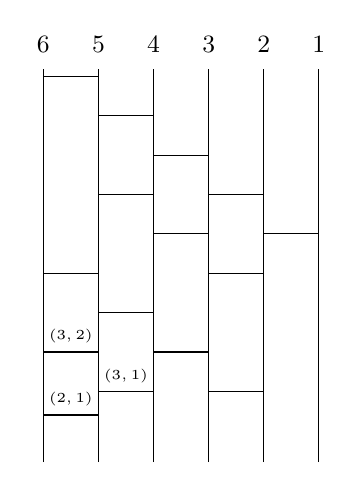
\begin{tikzpicture}
        \draw(0, 0) to (0, 5);
            \draw(0, 4.9) to (.7,4.9);
            \node at(.35, 1.6){\tiny{$(3,2)$}};
            \draw(0, 2.4) to (.7, 2.4);
            \node at(.35, 0.8){\tiny{$(2,1)$}};
            \draw(0, 1.4) to (.7, 1.4);
            \draw(0, .6) to (.7, .6);
        \draw(.7, 0) to (0.7, 5);
            \draw(.7, 4.4) to (1.4, 4.4);
            \draw(.7, 3.4) to (1.4, 3.4);
            \node at(1.05, 1.1){\tiny{$(3,1)$}};
           
            \draw(.7, 1.9) to (1.4, 1.9);
             \draw(.7, 0.9) to (1.4, 0.9);
        \draw(1.4, 0) to (1.4, 5);
            \draw(1.4, 3.9) to (2.1, 3.9);
            \draw(1.4, 2.9) to (2.1, 2.9);
            \draw(1.4, 1.4) to (2.1, 1.4);
        \draw(2.1, 0) to (2.1, 5);
            \draw(2.1, 3.4) to (2.8, 3.4);
            \draw(2.1, 2.4) to (2.8, 2.4);
            \draw(2.1, 0.9) to (2.8, 0.9);
        \draw(2.8, 0) to (2.8, 5);
            \draw(2.8, 2.9) to (3.5, 2.9);
        \draw(3.5, 0) to (3.5, 5);

        %%nodes
        \node at(0,5.3){\small{$6$}};
        \node at(0.7,5.3){\small{$5$}};
        \node at(1.4,5.3){\small{$4$}};
        \node at(2.1,5.3){\small{$3$}};
        \node at(2.8,5.3){\small{$2$}};
        \node at(3.5,5.3){\small{$1$}};
    \end{tikzpicture}
    \caption{A ladder with a clean level of $3$. All bars of the form $(a,3)$ where $a>3>c$ are above 
    $(3,c)$ and all of the bars of the form $(c,d)$ where $3>c>d$ are below $(3,d)$ $3$ is the maximum 
    element in $\pi$ from $1 \dots n-1$ where the above property holds.}
    \label{Fig:CleanLevel2}
\end{figure}
Given the route associated with $x$, each bar in $x's$ route requires its own row in the root ladder. In other words, 
no two bars in the route of $x$ share the same row. If $(x,y)$ exists and $(x,z)$ exists then  
$(x,y)$ is to the left of $(x,z)$ if and only if $R((x,y))<R((x,z))$. However, given $x$ and $y$ where $x \neq y$, a bar 
associated with $x$ can share a row with a bar associated with $y$ in the root ladder. Let $l_{i}$ be line $i$ in the ladder. The \emph{direction} of an element 
refers to an element crossing a bar connecting $l_{i}$ to $l_{i-1}$ or $l_{i+1}$. If an element crosses a bar going from 
from $l_{i}$ to $l_{i-1}$ then said element has a right-to-left direction. If an element crosses a bar 
from $l_{i}$ to $l_{i+1}$ then said element has a left-to-right direction. A \emph{switch in direction} refers 
to an elements direction switching from left-to-right or from right-to-left as said element travels 
along its path. If the maximum 
number of direction switches for any element is $>1$ then the ladder is not the root ladder of $OptL\{\pi\}$.  
In \ref{Fig:Route}, elements $1$ and $2$ have a right-to-left direction, element $3$ has a left-to-right direction, 
element $4$ starts with a right-to-left direction and then switches to a left-to-right direction, and element $5$ has a left-to-right direction. 
In the root ladder, as $x$ travels along the associated component of its route, the direction must be left-to-right. If $x$ travels 
along the unassociated component of its route, the direction must be right-to-left. 


Although unique, the root ladder can be drawn in many different ways due to the fact of ladder equivalency and ladder identity which were discussed in Chapter 1. 
For example, if one refers to Figure~\ref{Fig:RootLadderHeights}, one can see the root ladder for $(6,1,3,2,4,5)$ drawn in three different ways. 
Let the \emph{canonical configuration of the root ladder} be the representation of the root ladder with a height of $2(n-1)-1$. In Figure~\ref{Fig:RootLadderHeights}, 
the leftmost ladder is the canonical configuration of the root ladder because it has a height of $9=2(6-1)-1$. The reason $2(n-1)-1$ is chosen as the 
height of the canonical configuration of the root ladder is because any root ladder of order $n$ requires at most 
$2(n-1)-1$ rows by Theorem~\ref{Theorem:RootHeight} and Corollary~\ref{Corollary:RootHeight}. 
Therefore, when $2(n-1)-1$ is used as the height of the ladder, the two dimensional array used 
for solving the Canonical Ladder Listing Problem has static dimensions of $2(n-1)-1$ rows and $(n-1)$ columns.

\begin{theorem}
  The number of rows required for the root ladder corresponding to the descending permutation of order $n$ is $2(n-1) - 1$.
  \label{Theorem:RootHeight}
\end{theorem}
\begin{proof}
	Let $\pi$ be the descending permutation of order $n$. Let $Route(x)$ be the route associated with element $x$ in the corresponding root ladder of $\pi$. 
    Let $R(x)$ be the row of the uppermost, leftmost bar 
    of the route associated with $x \in \pi$. Let $R\prime(x)$ be the row of the bottommost, rightmost bar of the route associated 
    with $x \in \pi$. Let $C(x)$ be the column of the uppermost, leftmost bar of the route associated with $x \in \pi$.
    Let $C\prime(x)$ be the column of the bottommost, rightmost bar of the route associated $x \in \pi$. 
    For each $x \in \pi$, the number of inversions formed with $x$ such that $x$ is the greater of the two 
    elements in the inversion is $x-1$. Thus, in the corresponding root ladder 
    associated with $\pi$, $Route(x)$ has $x-1$ bars. Furthermore, 
    no bar in $Route(x)$ shares a row with any other bar in $Route(x)$ in the root ladder by the fourth property. Therefore, $Route(x)$ requires 
    $x-1$ rows. In the root ladder, $C(x)=1$ for each $x$ in $\pi$. This is true due to the fifth property, along with the fact that the number of 
    bars in $Route(x)$ is $x-1$. Since $Route(x)=x-1$, $C(x)=1$ and $x-1$ rows are 
    required for $Route(x)$, then $C'(x)=x-1$. If $x=n$ then $R(x)=1$, $C(x)=1$, $R\prime(x)=n-1$, and $C\prime(x)=n-1$. 
    If $1 < x < n$ then $R(x) = 2+R(x+1)$, $C(x)=1$, $R\prime(x)=1+R\prime(x+1)$ and $C\prime(x)=x-1$. There are $n-2$ elements 
    between $1$ and $n$. For all $1 < x < n$, $R\prime(x)$ is located one row below $R\prime(x+1)$, therefore one additional row 
    needs to be added to the ladder to accommodate the bottommost bar of the route associated with $x$. Thus, $n-2$ rows 
    need to be added to the ladder for each element $x$. The $nth$ element requires 
    $n-1$ rows for its route. Thus, there are $(n-1)+(n-2)=2(n-1)-1$ rows required for the root ladder corresponding to the descending permutation. 
\end{proof}

\begin{corollary}
    Let $ladder$ be the data structure for the root ladder for any permutation of order $n$. Let $r$ be the number of rows required 
    for $ladder$. Let $c$ be the number of columns required for $ladder$. $0 \leq r \leq 2(n-1)-1$ and $c=(n-1)$.
    \label{Corollary:RootHeight}
\end{corollary}
\begin{proof}
    By Theorem~\ref{Theorem:RootHeight}, we know that $r=2(n-1)-1$ for the root ladder corresponding 
    to the descending permutation of order $n$. The number of bars required for said ladder is $n \choose 2$. Let $b$ 
    be the number of bars required for any root ladder of order $n$. We know that when $b=n\choose2$, $r=2(n-1)-1$. By removing 
    bars from the root ladder for the descending permutation of order $n$, we can derive any other root ladder for any other permutation 
    of order $n$. Removing bars from the root ladder corresponding to the descending permutation of order $n$ 
    does not necessarily remove a row from $ladder$, however, removing bars from $ladder$ certainly does not add any more rows 
    to $ladder$. Therefore, $0 \leq r \leq 2(n-1)-1$. $c=(n-1)$ seeing as there are $n$ lines for any ladder of order $n$ and 
    a column is defined by a pair of lines.
\end{proof}



\begin{figure}
    \centering
    \begin{minipage}{0.3\textwidth}
	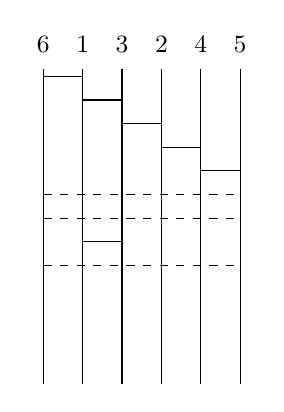
\begin{tikzpicture}

		\draw(0, 0) to (0, 4);
			\draw(0, 3.9) to (0.5, 3.9);
		\draw(0.5, 0) to (0.5, 4);
			\draw(0.5, 3.6) to (1, 3.6);
			\draw(0.5, 1.8) to (1, 1.8);
		\draw(1, 0) to (1, 4);
			\draw(1, 3.3) to (1.5, 3.3);
		\draw(1.5, 0) to (1.5, 4);
            \draw(1.5, 3.0) to (2, 3.0);
		\draw(2, 0) to (2, 4);
            \draw(2, 2.7) to (2.5, 2.7);
		\draw(2.5, 0) to (2.5, 4);
        \draw[dashed](0, 2.4) -- (2.5, 2.4);
        \draw[dashed](0, 2.1) -- (2.5, 2.1);
        \draw[dashed](0, 1.5) -- (2.5, 1.5);


		\node at(0, 4.3){\small{$6$}};
		\node at(0.5, 4.3){\small{$1$}};
		\node at(1, 4.3){\small{$3$}};
		\node at(1.5, 4.3){\small{$2$}};
		\node at(2, 4.3){\small{$4$}};
		\node at(2.5, 4.3){\small{$5$}};
		
	\end{tikzpicture}
  
    \end{minipage}
    \begin{minipage}{0.3\textwidth}
	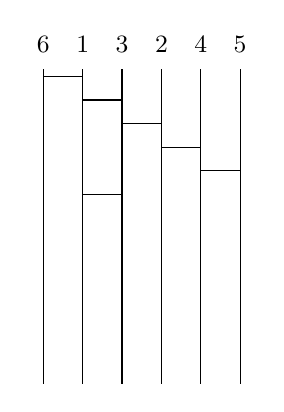
\begin{tikzpicture}

		\draw(0, 0) to (0, 4);
			\draw(0, 3.9) to (0.5, 3.9);
		\draw(0.5, 0) to (0.5, 4);
			\draw(0.5, 3.6) to (1, 3.6);
			\draw(0.5, 2.4) to (1, 2.4);
		\draw(1, 0) to (1, 4);
			\draw(1, 3.3) to (1.5, 3.3);
		\draw(1.5, 0) to (1.5, 4);
            \draw(1.5, 3.0) to (2, 3.0);
		\draw(2, 0) to (2, 4);
            \draw(2, 2.7) to (2.5, 2.7);
		\draw(2.5, 0) to (2.5, 4);


		\node at(0, 4.3){\small{$6$}};
		\node at(0.5, 4.3){\small{$1$}};
		\node at(1, 4.3){\small{$3$}};
		\node at(1.5, 4.3){\small{$2$}};
		\node at(2, 4.3){\small{$4$}};
		\node at(2.5, 4.3){\small{$5$}};
		
	\end{tikzpicture}
    \end{minipage}
    \begin{minipage}{0.3\textwidth}
	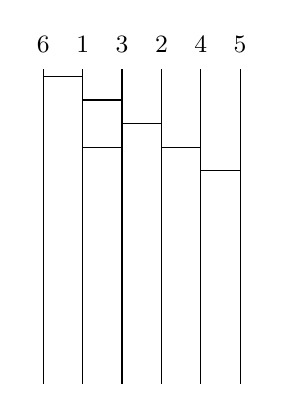
\begin{tikzpicture}

		\draw(0, 0) to (0, 4);
			\draw(0, 3.9) to (0.5, 3.9);
		\draw(0.5, 0) to (0.5, 4);
			\draw(0.5, 3.6) to (1, 3.6);
			\draw(0.5, 3.0) to (1, 3.0);
		\draw(1, 0) to (1, 4);
			\draw(1, 3.3) to (1.5, 3.3);
		\draw(1.5, 0) to (1.5, 4);
            \draw(1.5, 3.0) to (2, 3.0);
		\draw(2, 0) to (2, 4);
            \draw(2, 2.7) to (2.5, 2.7);
		\draw(2.5, 0) to (2.5, 4);


		\node at(0, 4.3){\small{$6$}};
		\node at(0.5, 4.3){\small{$1$}};
		\node at(1, 4.3){\small{$3$}};
		\node at(1.5, 4.3){\small{$2$}};
		\node at(2, 4.3){\small{$4$}};
		\node at(2.5, 4.3){\small{$5$}};
		
	\end{tikzpicture}
    \end{minipage}
      \caption{All three root ladders are equivalent. The left and middle ladder are identical, 
      with 6 rows each. The height of the left ladder is 9, the height of the middle ladder is 6, and the height of the right ladder is 5.}
      \label{Fig:RootLadderHeights}
\end{figure}


\begin{lemma}
    If $x$ has bars associated with its route, then the bottommost bar of the route of $x$ 
    is associated with the route of $x$ in the root ladder.
    \label{Proof:RouteAssociation}
\end{lemma}
\begin{proof}
    We shall do a proof by contradiction. Let $w>x>y \in \pi$. Let $p_{w}<p_{x}<_p_{y}$. Let $(w,x)$ be the bottommost bar of $x's$ route. 
    We know $x$ crosses $(w,x)$ from the right-to-left. 
    $x$ has route association, therefore $(x,y)$ is a bar and we 
    know $x$ crosses $(x,y)$ from left-to-right. 
    Since $(w,x)$ and $(x,y)$ exist, so does $(w,y)$. From our assumption, we assumed $(w,x)$ was the bottommost bar of 
    $x's$ route. Therefore, $R((x,y))<R((w,x))$. $R((w,y)) < R((x,y))$ due the root ladder having a clean level of $1$. 
    Therefore, $R((w,y))<R((w,x))$. Yet, $p_{w}<p_{x}<p_{y}$  Therefore, 
    $R((w,x))<R((w,y))$. Contradiction. Therefore, the bottommost bar of the route of $x$ must be associated with $x$. 
    
\end{proof}
\begin{corollary}
    If $x$ has bars associated with its route, then the column of the bottommost bar of the route of $x$ is column $x-1$.
    \label{Corollary:Column}
\end{corollary}
\begin{proof}
    Let $b$ be the bottommost bar of the route of $x$. From Lemma~\ref{Proof:RouteAssociation} we know that $b$ is associated 
    with $x$. Therefore, $x$ crosses $b$ from left-to-right. We also know that $x$ must end up at the bottom of line $x$. 
    Let $c$ be the $x-1$ column in the root ladder. Let $l_{x}$ be line $x$ in the ladder. Conceptually, $c$ is the gap between $l_{x-1}$ 
    and $l_{x}$. Since $x$ crosses $b$ from left to right and $x$ must end at line $x$, $b$ must be located at column $x-1$.    
\end{proof}
 

We use Corollary~\ref{Corollary:RootHeight}, Corollary~\ref{Corollary:Column}, and the properties of the root 
ladder to derive a naive algorithm for creating the canonical configuration of any root ladder corresponding to 
any permutation of order $n$.
In order to view said algorithm, please refer to Algorithm~\ref{Alg:RootLadder}. 
The initial conditions of Algorithm~\ref{Alg:RootLadder} are the 
following. Let $ladder$ be initialized to an empty ladder. Let $\pi$ be an arbitrary permutation 
of order $n$. Let $x$ be the current element in $\pi$ initialized to $n$.
\begin{algorithm}[ht]
	\begin{algorithmic}[1]
		\Function {CreateRoot}{$ladder$, $\pi$, $x$}
			\If{$x=1$}
				\State \textbf{return}
            \EndIf
            \State $index \gets p_{x}$
            \State $numBars \gets x-index$
            \State $col \gets x-1$
            \State $row \gets (n-1)+(n-x)$
            \For{$i \gets 1$ \textbf{to} $numBars$}
                    \State $ladder[row][col] \gets 1$
                    \State $row \gets row-1$
                    \State $col \gets col-1$
            \EndFor
            \State $\pi \gets \pi - x$
            \State {\sc CreateRoot($ladder$, $\pi$, $n$, $x-1$)}
        \EndFunction

	\end{algorithmic}
	\caption{The algorithm for creating the root ladder of $OptL\{\pi\}$}
	\label{Alg:RootLadder}
\end{algorithm}

Bars associated with the route of the $xth$ element are added, starting 
from the bottommost bar to the topmost bar. Once all the bars 
for the associated route of the $xth$ element have been added, the function makes a recursive call. Just prior to the recursive 
call, element $x$ is removed from $\pi$; all the elements to the left of element $x$ in $\pi$ 
maintain their same index, and all the elements to the right of element $x$ in $\pi$ are moved one index to the left in $\pi$. 
On the recursive call, $x$ is decremented by $1$; this ensures that $x$ is always the maximal element in $\pi$. 
The local variable $numBars$ 
represents the number of bars associated with the route of $x$. On each recursive call $x$ is always the largest element in $\pi$, 
thus the number of 
inversions associated with $x$, such that $x$ is the larger element of said inversion, equals 
$x$ minus the position of element $x$ in $\pi$. Therefore, the number of bars associated with the route of $x$ equals $x-p_{x}$.\par 
The local variable $col$ represents the column to place the bottommost bar associated with 
the route of $x$. By Corollary~\ref{Corollary:Column}, it has been shown that $col=x-1$. The local variable $row$ represents 
the row to place the bottommost bar associated with the route of $x$. When $x=n$, the maximum number of 
bars associated with $x$ for any permutation of order $n$ is $n-1$. 
Therefore, the bottommost bar of route $x$, when $x=n$, is by default placed at row $n-1$. 
Once $row$ is initialized to $(n-1)$, $row$ will be incremented by an offset value of $(n-x)$. Conceptually, the offset increment means that the row for the bottommost bar associated with the route of $x$ is one 
greater than the row for the bottommost bar associated with element $x+1$.  
To see the resulting state of $ladder$ for each recursive call to {\sc CreateRoot} with $\pi=(5,7,3,4,1,2,6)$ please refer to Figure~\ref{Fig:CreateRoot}\pagebreak

\begin{figure}[t]
    \centering 
    \begin{minipage}{.3\textwidth}
    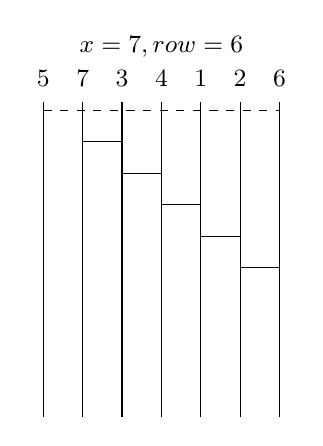
\begin{tikzpicture}
        \draw(0, 0) to (0, 4);
        
        \draw(.5, 0) to (.5, 4);
        \draw(1, 0) to (1, 4);
        \draw(1.5, 0) to (1.5, 4);
        \draw(2, 0) to (2, 4);
        \draw(2.5, 0) to (2.5, 4);
        \draw(3, 0) to (3, 4);
        
        \draw(2.5, 1.9) to (3, 1.9);
        \draw(2.0, 2.3) to (2.5, 2.3);
        \draw(1.5, 2.7) to (2.0, 2.7);
        \draw(1.0, 3.1) to (1.5, 3.1);
        \draw(0.5, 3.5) to (1.0, 3.5);

        \draw[dashed] (0, 3.9) -- (3, 3.9);
        \node at(1.5, 4.7){\small{$x=7,row=6$}};
        \node at(0, 4.3){\small{$5$}};
        \node at(.5, 4.3){\small{$7$}};
        \node at(1, 4.3){\small{$3$}};
        \node at(1.5, 4.3){\small{$4$}};
        \node at(2, 4.3){\small{$1$}};
        \node at(2.5, 4.3){\small{$2$}};
        \node at(3, 4.3){\small{$6$}};
    \end{tikzpicture}
    \end{minipage}
    \begin{minipage}{.3\textwidth}
    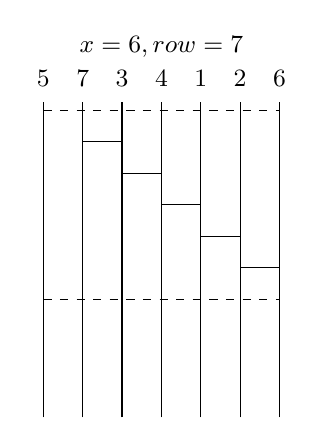
\begin{tikzpicture}
        \draw(0, 0) to (0, 4);
        \draw(.5, 0) to (.5, 4);
        \draw(1, 0) to (1, 4);
        \draw(1.5, 0) to (1.5, 4);
        \draw(2, 0) to (2, 4);
        \draw(2.5, 0) to (2.5, 4);
        \draw(3, 0) to (3, 4);
        
        \draw[dashed] (0, 3.9) -- (3, 3.9);
        \draw[dashed] (0, 1.5) -- (3, 1.5);
        \draw(2.5, 1.9) to (3, 1.9);
        \draw(2.0, 2.3) to (2.5, 2.3);
        \draw(1.5, 2.7) to (2.0, 2.7);
        \draw(1.0, 3.1) to (1.5, 3.1);
        \draw(0.5, 3.5) to (1.0, 3.5);

        \node at(1.5, 4.7){\small{$x=6,row=7$}};

        \node at(0, 4.3){\small{$5$}};
        \node at(.5, 4.3){\small{$7$}};
        \node at(1, 4.3){\small{$3$}};
        \node at(1.5, 4.3){\small{$4$}};
        \node at(2, 4.3){\small{$1$}};
        \node at(2.5, 4.3){\small{$2$}};
        \node at(3, 4.3){\small{$6$}};
    \end{tikzpicture}
    \end{minipage}
   \begin{minipage}{.3\textwidth}
    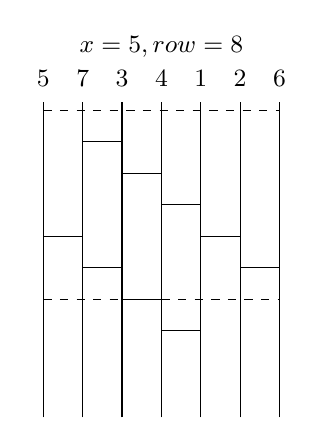
\begin{tikzpicture}
        \draw(0, 0) to (0, 4);
            \draw(0, 2.3) to (0.5, 2.3);
        \draw(.5, 0) to (.5, 4);
            \draw(.5, 1.9) to (1, 1.9);
        \draw(1, 0) to (1, 4);
            \draw(1, 1.5) to (1.5, 1.5);
        \draw(1.5, 0) to (1.5, 4);
            \draw(1.5, 1.1) to (2, 1.1);
            \draw(1.5, 2.7) to (2, 2.7);
        \draw(2, 0) to (2, 4);
        \draw(2.5, 0) to (2.5, 4);
        \draw(3, 0) to (3, 4);
        \draw[dashed] (0, 3.9) -- (3, 3.9);


        \draw(2.5, 1.9) to (3, 1.9);
        \draw(2.0, 2.3) to (2.5, 2.3);

        \draw(1.0, 3.1) to (1.5, 3.1);
        \draw(0.5, 3.5) to (1.0, 3.5);
      
        \draw[dashed] (0, 1.5) -- (1, 1.5);
        \draw[dashed] (1.5, 1.5) -- (3, 1.5);
        

        \node at(1.5, 4.7){\small{$x=5,row=8$}};
        \node at(0, 4.3){\small{$5$}};
        \node at(.5, 4.3){\small{$7$}};
        \node at(1, 4.3){\small{$3$}};
        \node at(1.5, 4.3){\small{$4$}};
        \node at(2, 4.3){\small{$1$}};
        \node at(2.5, 4.3){\small{$2$}};
        \node at(3, 4.3){\small{$6$}};
    \end{tikzpicture}
    \end{minipage}
        
    \begin{minipage}{.3\textwidth}
    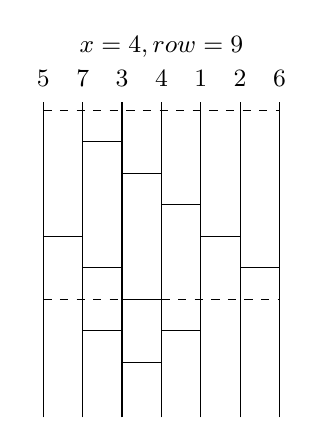
\begin{tikzpicture}
    \draw(0, 0) to (0, 4);
            \draw(0, 2.3) to (0.5, 2.3);
        \draw(.5, 0) to (.5, 4);
            \draw(.5, 1.9) to (1, 1.9);
            \draw(0.5, 1.1) to (1, 1.1);
        \draw(1, 0) to (1, 4);
            \draw(1, 1.5) to (1.5, 1.5);
            \draw(1, 0.7) to (1.5, 0.7);
        \draw(1.5, 0) to (1.5, 4);
            \draw(1.5, 1.1) to (2, 1.1);
            \draw(1.5, 2.7) to (2, 2.7);
        \draw(2, 0) to (2, 4);
        \draw(2.5, 0) to (2.5, 4);
        \draw(3, 0) to (3, 4);
        \draw[dashed] (0, 3.9) -- (3, 3.9);


        \draw(2.5, 1.9) to (3, 1.9);
        \draw(2.0, 2.3) to (2.5, 2.3);

        \draw(1.0, 3.1) to (1.5, 3.1);
        \draw(0.5, 3.5) to (1.0, 3.5);
      
        \draw[dashed] (0, 1.5) -- (1, 1.5);
        \draw[dashed] (1.5, 1.5) -- (3, 1.5);
        

        \node at(1.5, 4.7){\small{$x=4,row=9$}};
        \node at(0, 4.3){\small{$5$}};
        \node at(.5, 4.3){\small{$7$}};
        \node at(1, 4.3){\small{$3$}};
        \node at(1.5, 4.3){\small{$4$}};
        \node at(2, 4.3){\small{$1$}};
        \node at(2.5, 4.3){\small{$2$}};
        \node at(3, 4.3){\small{$6$}};
    \end{tikzpicture}
    \end{minipage}
    \begin{minipage}{.3\textwidth}
    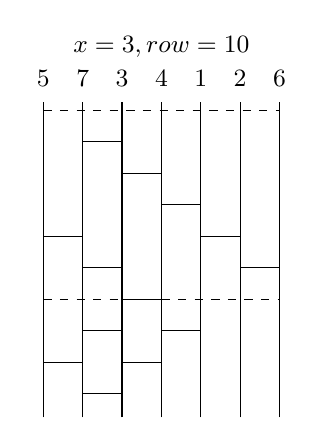
\begin{tikzpicture}
     \draw(0, 0) to (0, 4);
            \draw(0, 2.3) to (0.5, 2.3);
            \draw(0, 0.7) to (0.5, 0.7);
        \draw(.5, 0) to (.5, 4);
            \draw(.5, 1.9) to (1, 1.9);
            \draw(0.5, 1.1) to (1, 1.1);
            \draw(0.5, 0.3) to (1, 0.3);
        \draw(1, 0) to (1, 4);
            \draw(1, 1.5) to (1.5, 1.5);
            \draw(1, 0.7) to (1.5, 0.7);
        \draw(1.5, 0) to (1.5, 4);
            \draw(1.5, 1.1) to (2, 1.1);
            \draw(1.5, 2.7) to (2, 2.7);
        \draw(2, 0) to (2, 4);
        \draw(2.5, 0) to (2.5, 4);
        \draw(3, 0) to (3, 4);
        \draw[dashed] (0, 3.9) -- (3, 3.9);


        \draw(2.5, 1.9) to (3, 1.9);
        \draw(2.0, 2.3) to (2.5, 2.3);

        \draw(1.0, 3.1) to (1.5, 3.1);
        \draw(0.5, 3.5) to (1.0, 3.5);
      
        \draw[dashed] (0, 1.5) -- (1, 1.5);
        \draw[dashed] (1.5, 1.5) -- (3, 1.5);
        

        \node at(1.5, 4.7){\small{$x=3,row=10$}};
        \node at(0, 4.3){\small{$5$}};
        \node at(.5, 4.3){\small{$7$}};
        \node at(1, 4.3){\small{$3$}};
        \node at(1.5, 4.3){\small{$4$}};
        \node at(2, 4.3){\small{$1$}};
        \node at(2.5, 4.3){\small{$2$}};
        \node at(3, 4.3){\small{$6$}};
    \end{tikzpicture}
    \end{minipage}
    \begin{minipage}{.3\textwidth}
   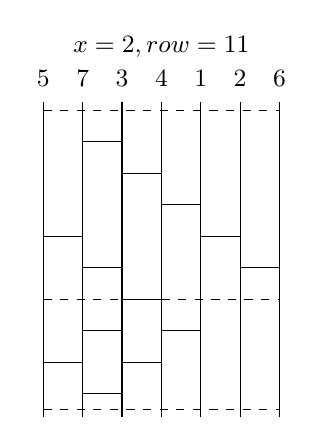
\begin{tikzpicture}
     \draw(0, 0) to (0, 4);
            \draw(0, 2.3) to (0.5, 2.3);
            \draw(0, 0.7) to (0.5, 0.7);
        \draw(.5, 0) to (.5, 4);
            \draw(.5, 1.9) to (1, 1.9);
            \draw(0.5, 1.1) to (1, 1.1);
            \draw(0.5, 0.3) to (1, 0.3);
        \draw(1, 0) to (1, 4);
            \draw(1, 1.5) to (1.5, 1.5);
            \draw(1, 0.7) to (1.5, 0.7);
        \draw(1.5, 0) to (1.5, 4);
            \draw(1.5, 1.1) to (2, 1.1);
            \draw(1.5, 2.7) to (2, 2.7);
        \draw(2, 0) to (2, 4);
        \draw(2.5, 0) to (2.5, 4);
        \draw(3, 0) to (3, 4);
        \draw[dashed] (0, 3.9) -- (3, 3.9);


        \draw(2.5, 1.9) to (3, 1.9);
        \draw(2.0, 2.3) to (2.5, 2.3);

        \draw(1.0, 3.1) to (1.5, 3.1);
        \draw(0.5, 3.5) to (1.0, 3.5);
      
        \draw[dashed] (0, 1.5) -- (1, 1.5);
        \draw[dashed] (1.5, 1.5) -- (3, 1.5);
        

        \node at(1.5, 4.7){\small{$x=2,row=11$}};
        \node at(0, 4.3){\small{$5$}};
        \node at(.5, 4.3){\small{$7$}};
        \node at(1, 4.3){\small{$3$}};
        \node at(1.5, 4.3){\small{$4$}};
        \node at(2, 4.3){\small{$1$}};
        \node at(2.5, 4.3){\small{$2$}};
        \node at(3, 4.3){\small{$6$}};

        \draw[dashed](0, 0.1) -- (3, 0.1);
    \end{tikzpicture}
    \end{minipage}
    

        
        % \node at(9.5, -5.3){\small{$x=2,row=10$}};

        % \node at(0, -.7){\small{$5$}};
        % \node at(.5, -.7){\small{$7$}};
        % \node at(1, -.7){\small{$3$}};
        % \node at(1.5, -.7){\small{$4$}};
        % \node at(2, -.7){\small{$1$}};
        % \node at(2.5, -.7){\small{$2$}};
        % \node at(3, -.7){\small{$6$}};
        
        % \node at(4, -.7){\small{$5$}};
        % \node at(4.5, -.7){\small{$7$}};
        % \node at(5, -.7){\small{$3$}};
        % \node at(5.5, -.7){\small{$4$}};
        % \node at(6, -.7){\small{$1$}};
        % \node at(6.5, -.7){\small{$2$}};
        % \node at(7, -.7){\small{$6$}};

        % \node at(8, -.7){\small{$5$}};
        % \node at(8.5, -.7){\small{$7$}};
        % \node at(9, -.7){\small{$3$}};
        % \node at(9.5, -.7){\small{$4$}};
        % \node at(10, -.7){\small{$1$}};
        % \node at(10.5, -.7){\small{$2$}};
        % \node at(11, -.7){\small{$6$}};
        
    
    \caption{The ordering of the state of the ladder when creating the root ladder for $(5,7,3,4,1,2,6)$}
    \label{Fig:CreateRoot}
\end{figure}

\begin{lemma}
	The time complexity for CreateRoot is $O(n^{2})$
\end{lemma}
\begin{proof}
	The for-loop runs from some arbitrary index to $n$ on each function call. Thus, we get $O(n)$. The following 
    recursion holds, $CreateRoot(n-k) = CreateRoot((n-k)+1) + n=CreateRoot((n-k)+2) + n-1\dots $. The recurrence 
    relation is reduced to $n(n+1)/2= O(n^2)$.
\end{proof}


We could use the naive algorithm to list $L_{n}$, however, doing so is rather inefficient. 
In the proceeding sections of Chapter 3, we provide the {\sc ModifiedSJT} and {\sc CyclicBar} algorithms in order to list $L_{n}$. 
{\sc ModifiedSJT} and {\sc CyclicBar} require additional auxiliary functions. We define {\sc Inv(x)} as follows: $|\forall y \in \pi : y < x, p_{y}>p_{x}|$. 
For example, given $(3,4,1,5,6,2)$, {\sc Inv(1)=0}, {\sc Inv(2)=0}, {\sc Inv(3)=2}, {\sc Inv(4)=2}, {\sc Inv(5)=1}, {\sc Inv(6)=1}. 
Given {\sc Inv(x)}, 
we can define the function {\sc GetCoordinates}. In order to define {\sc GetCoordinates}, let $x>y \in \pi$. Given 
$p_{x}$ and $p_{y}$, suppose a transposition were applied to $x$ and $y$. Prior to the transposition 
of $x$ and $y$, if $p_{x} = p_{y}-1$ then {\sc GetCoordinates} returns the row and column of the bar $(x,y)$ to be removed 
from the ladder. If $p_{x}=p_{y}+1$, then {\sc GetCoordinates} returns 
the row and column of bar $(x,y)$ to be added to the ladder. 





